%\chapter{Utility AI}
\label{chap:utilityai}

\section{Idea Of Utility AI}
\label{sec:utilityai_ideaofutilityai}

The main goal of utility AI is to give NPCs more dynamic behaviour while keeping everything simple to read and understand. The general idea has been around for a while, but has been given a remarkable push by Dave Mark, president and lead designer of Intrinsic Algorithm LLC. Utility AI is about giving NPCs some information and possible actions, and then letting them decide for themselves what is the best action to take given the current circumstances. The goal is to make the AI feel alive and responsive by doing a very simplified version of what humans do when making a decision: Evaluate the circumstances and choose the best resulting action. \cite{UtilityAiFunctionality}

The way utility AI works is that the NPC has a predefined set of possible states, and each time it decides what to do next, it evaluates all the states based on their associated considerations. A consideration is just some information about the environment. The state with the highest score is then executed next, causing the NPC to take action.

\section{Terminology}
\label{sec:utilityai_terminology}

To avoid confusion between the different aspects of utility AI, the following terminology is used in this paper:

\begin{tabular}{lp{12cm}}
State Set: & A simple container of states to help organise the states and allow runtime changes to state sets. \cr
State: & A state that the NPC can be in. While in a state, the NPC performs a task as defined in the state's behaviour tree. It has two other components: preconditions and evaluators, which are responsible for calculating the state's score. \cr
Precondition: & Each state can have any number of preconditions. If a precondition is not met, the state will not be selected, regardless of its score. \cr
Evaluator: & Each consideration can optionally be associated with an evaluator, which will then score it using an adjustable curve. \cr
Consideration: & The NPC's knowledge of his needs and his environment. Its value can change over time and is used as input for evaluating states. \cr
Weight: & Evaluators and actions each have their own weight. It can be used to change the NPC's overall preferences. \cr
Score: & The utility NPC's scoring system, used to decide the best state.
\end{tabular}

\section{How It Works}
\label{sec:utilityai_howitworks}
\subsection{General Principle}
\label{subsec:utilityai_howitworks_generalprinciple}

A state set contains several states, which are iterated through to evaluate the score of each and then select the one with the highest score.

\begin{figure}[H]
	\centering
		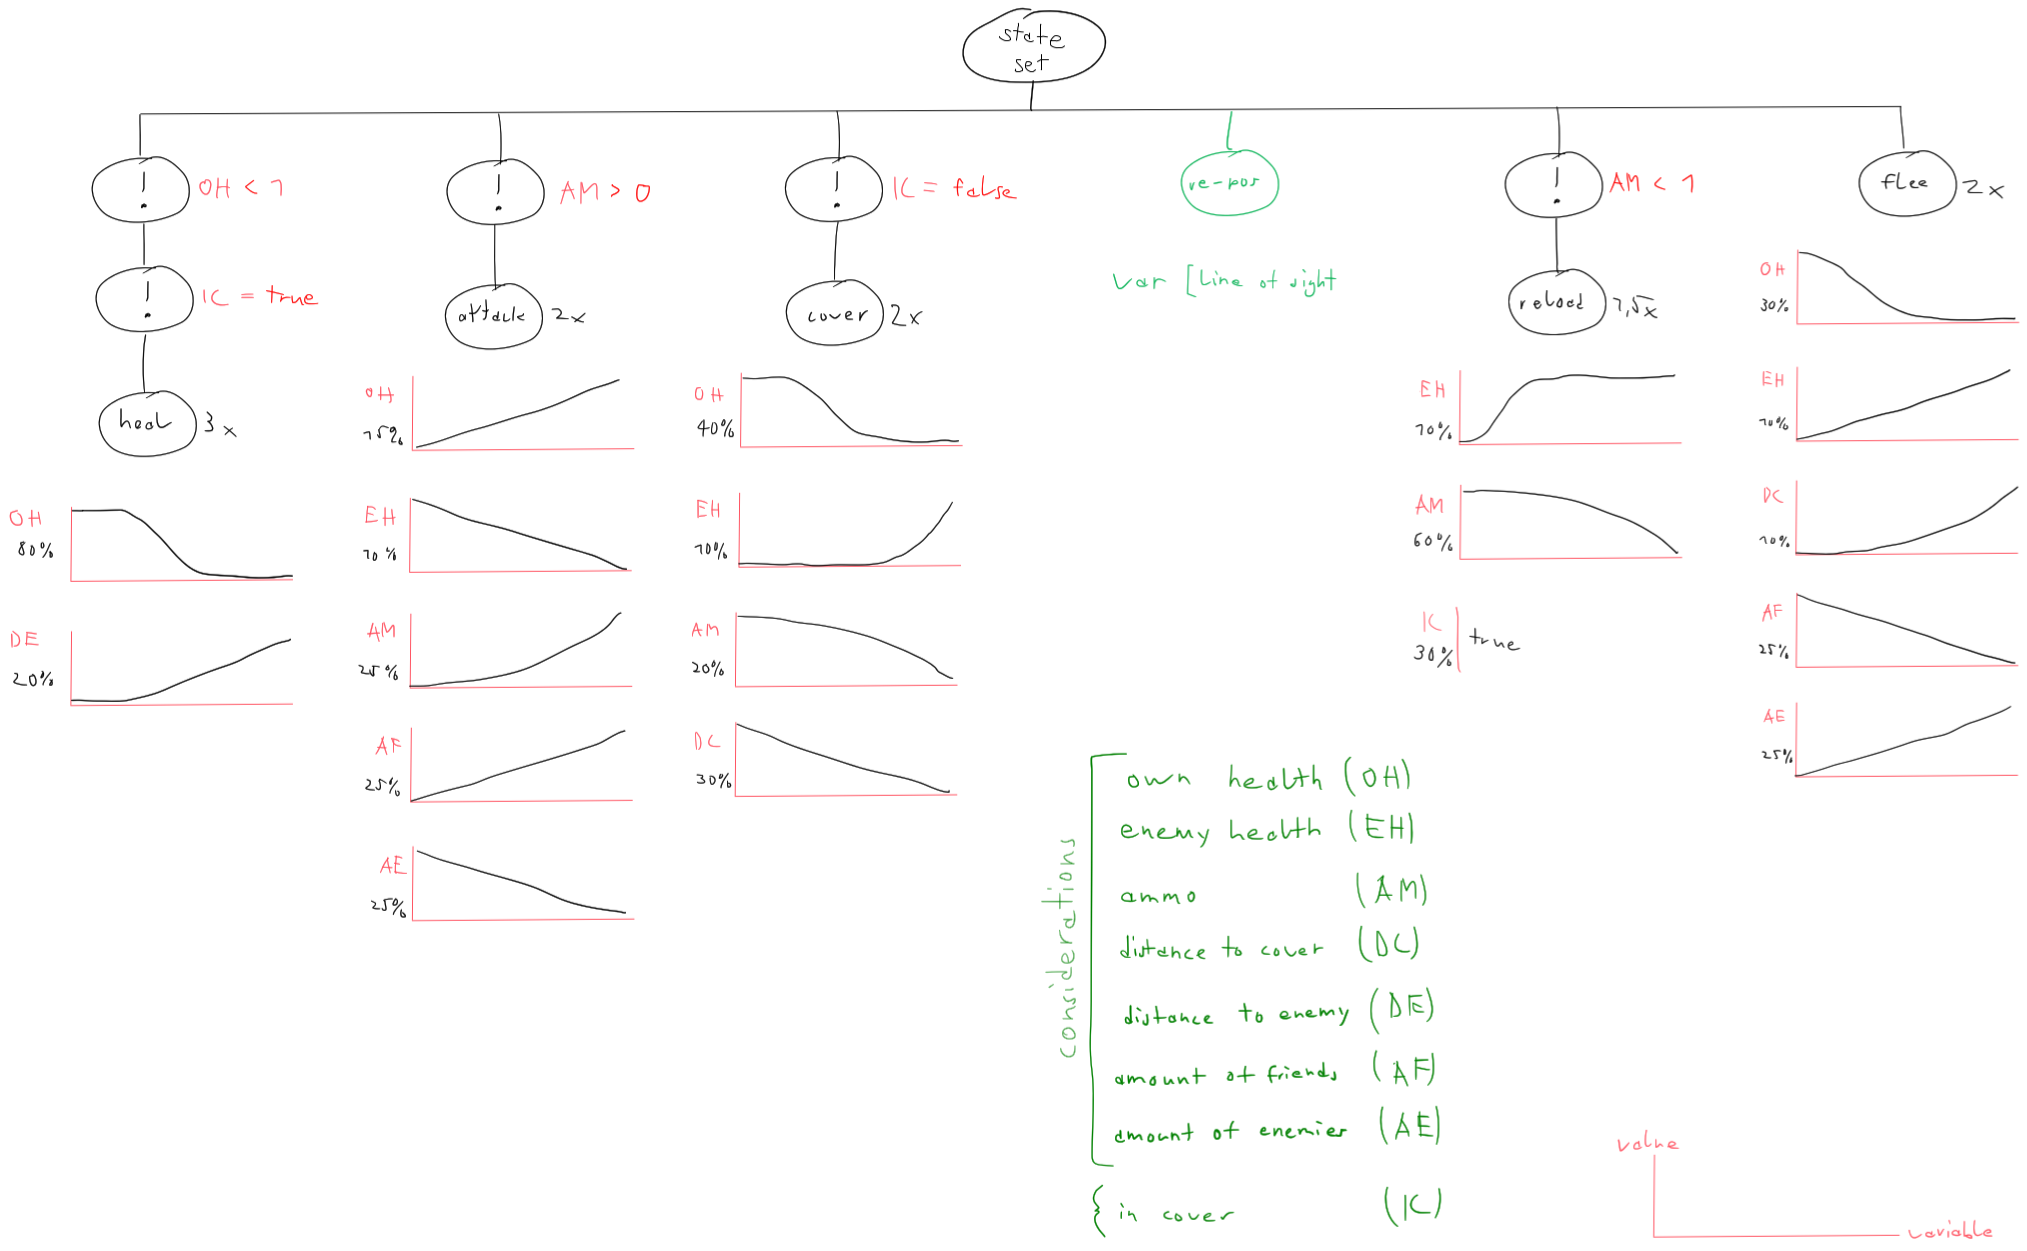
\includegraphics[scale=0.29]{images/utility_ai_sketch_defending_ai.png}
	\caption{Sketch of a defending NPC, using utility AI}
	\label{fig:utility_ai_sketch_defending_ai}
\end{figure}

This is the structure of an example scenario for a utility AI. It shows the behaviour of an agent trying to defend its territory against intruders.

As an example, below the "heal" state on the left are two curves representing the evaluators. For the first curve, the OH (own health) consideration is evaluated and scored from 0 to 1 based on the function of the curve with own health as the input parameter. The score is then multiplied by its weight, in this case 0.8. The same is done for the DE (distance to enemy) consideration.

All the scores from the evaluators will return a sum less than 1. This sum is then multiplied by the weight of the state, in the case of "heal" it would be multiplied by three.

A state will only be considered if each condition is met. In the "heal" example, the OH (own health) consideration must be less than 1 and the agent must be in cover, otherwise the state will be ignored.

The same procedure is then performed for each state that is in the state set.

\newpage

\subsection{Calculation Of The Score}
\label{subsec:utilityai_howitworks_calculationofthescore}

Dave Mark used a different formula to the one used in this paper. In his formula, all the scores from the evaluators are multiplied together, which then gives the total score. Since multiplying decimals will continuously make them smaller, he applies an averaging scheme to each action after it has received its score to compensate for this.

\begin{equation}
ActionScore = Score + \left(1 - Score\right) \cdot \left(1 - \frac{1}{TotalConsiderations}\right) \cdot Score
\end{equation}

This formula works for calculating the average score, but there is still a problem that might want to be avoided for certain scenarios. If one of the considerations scores 0 or close to 0, the final score will also be 0 or close to 0, no matter how well the other considerations score. \cite{UtilityAiTalk}

In the figure \ref{fig:utility_ai_sketch_defending_ai_with_values}, for example, if the evaluator for EH (enemy health) returns 0, the agent would never reload, no matter how little ammo was left in its weapon. Obviously this isn't the desired behaviour, unless a consideration is not allowed to be 0 for the state to work, but in this case a precondition could be used.

To overcome this problem, all the scores are instead added together and then divided by the total number of scores used. This approach is also simpler because it doesn't require an averaging scheme, so it's more intuitive to work with.

Up to here, the scores have simply been averaged without any weights. In order to add weight to the formula, the most straightforward solution is to give each evaluator a percentage representing its importance. Each score is then multiplied by this percentage before being added to the total score. A visualisation of this idea can be seen in the figure \ref{fig:utility_ai_sketch_defending_ai_with_values}.

Calculating the weight in this way introduces a new problem. If a new evaluator is added later, all the previous weights must be adjusted because the total percentage must be 100\%.

To address this issue, the weight of each evaluator is not set as a percentage, but as a decimal between 0 and 1. The corresponding percentage is then calculated in the background by dividing its weight by the sum of all weights. This way the weight of each consideration doesn't need to be changed when a new weight is added. The following equation is used to obtain the total score of a state:

\begin{equation}
TotalScore = StateWeight \cdot (BaseScore + \sum_{i=1}^{n} \left( Score_i \cdot \frac{EvalWeight_i}{TotalEvalWeights} \right))
\end{equation}

where \textit{n} is a list of all evaluators, and \textit{TotalEvalWeights} the sum of all weights from the evaluators of the state. The \textit{StateWeight} represents the weight that can be manually adjusted to change the overall importance of the state, as seen in the example figure \ref{fig:utility_ai_sketch_defending_ai_with_values} to the right of each state.

Each state also has a custom \textit{BaseScore} which is simply added before being multiplied by the \textit{StateWeight}. There is also the option to clamp the \textit{TotalScore} between two custom defined values.

A further problem arises when two states have almost identical scores, which can lead to the agent constantly switching between them. To prevent this, the current action has a bonus factor that can be set individually. This bonus factor is multiplied by the score of the state if it is the state currently being executed. This factor should be greater than one, for example 1.5, to give the current state a higher rating.

\subsection{Example Scenario}
\label{subsec:utilityai_howitworks_generalprinciple}

\begin{figure}[H]
    \centering
    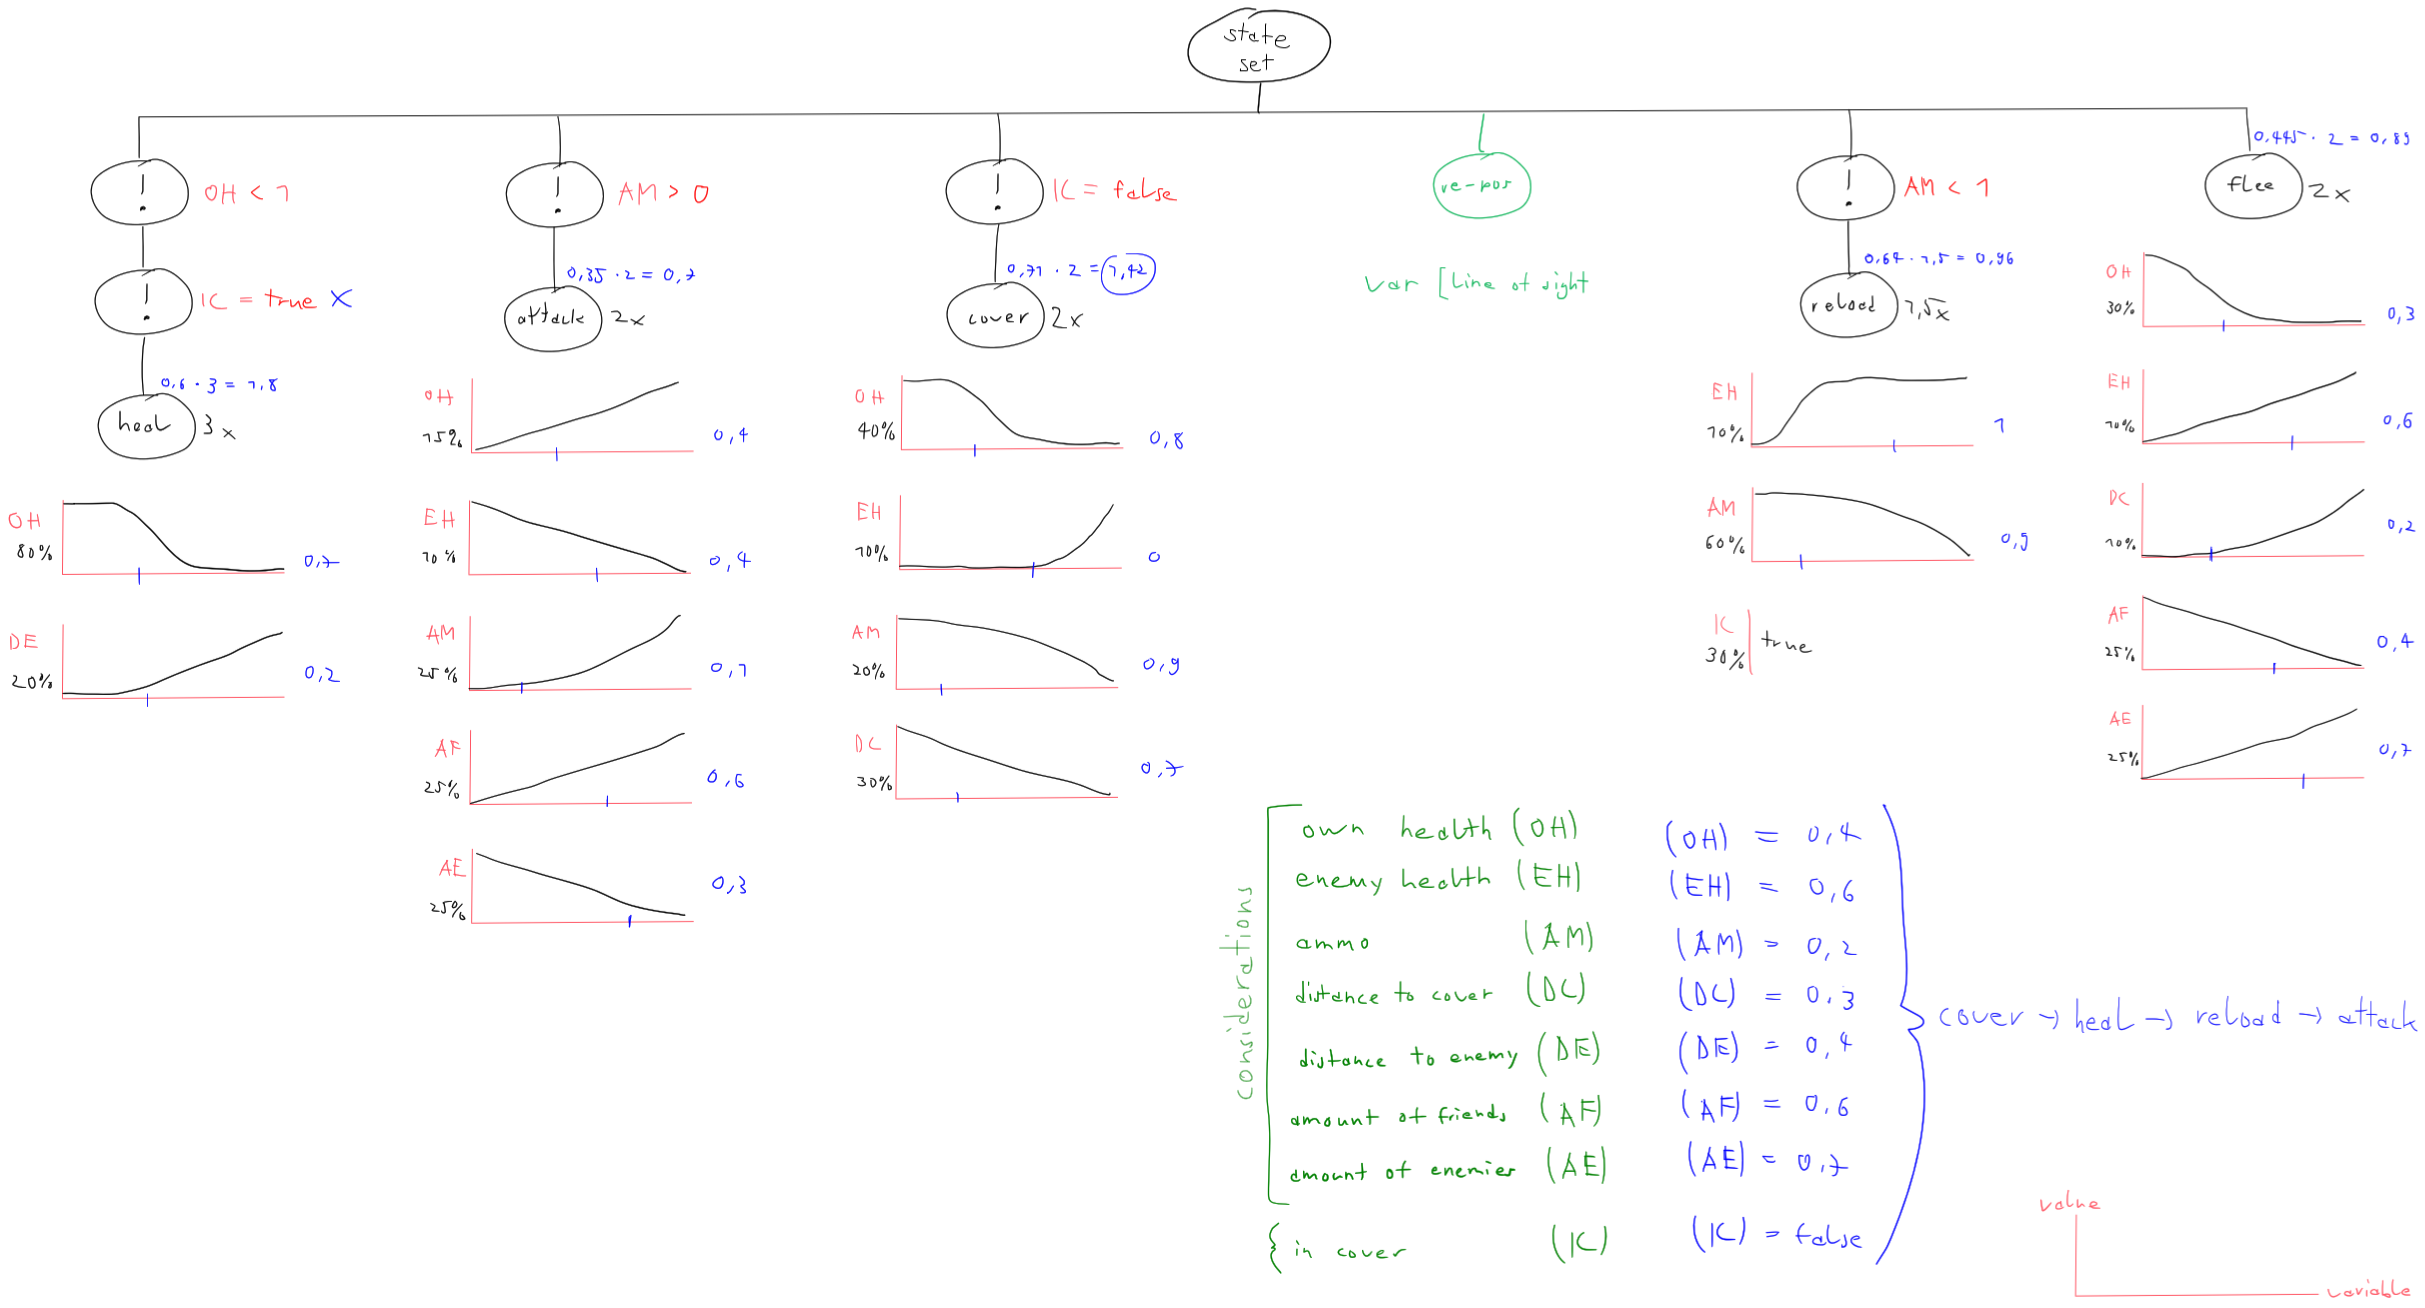
\includegraphics[scale=0.345, angle=90]{images/utility_ai_sketch_defending_ai_with_values.png}
    \caption{Sketch of a defending NPC, using utility AI and with example values}
    \label{fig:utility_ai_sketch_defending_ai_with_values}
\end{figure}

To better illustrate the idea of utility AI evaluation, some sample values have been chosen for all considerations to represent a possible state of the game.

Next to each evaluator is a number in blue, which represents the resulting value of the curve, given its respective consideration. The sum of these, together with the sum multiplied by the weight of the state, can be found next to each state.

In this particular scenario, the "heal" state has the highest score, but because one of its preconditions is not met, it is ignored. "cover" has the second highest score, and since all of its preconditions are met, it is selected as the next state.

Once the agent has reached cover, the next state to be executed is "heal", as it now fulfils all its requirements and still has the highest score.

After healing, the agent will most likely reload its weapon and then start attacking. The order of states may change as the game progresses. For example, if the agent gets badly injured while reloading, it will be less likely to attack. It all depends on the current state of reasoning.

\section{Example Implementations}
\label{sec:utilityai_exampleimplementations}
\subsection{Main Goal Of The Implementations}
\label{subsec:utilityai_realization_maingoaloftheimplementations}

Because the idea of utility AI isn't very well known, and also because the implementation used here differs in some ways from Dave Mark's, the concept needs to be tested first. To do this, a proof of concept was created in the Unity game engine, as it is one of the most popular game engines and supports the creation of new frameworks very well.

These quick implementations ar for proof-of-concept purposes only, and are not optimised for use in real projects. The easiest way to prove that utility AI works as expected is to create a simple framework for utility AI, and then create some example scenes that show its application. This way it is easy to see if utility AI makes sense in these scenarios, and if it does not, some adjustments can be made before spending a lot of time creating a tool, which mainly uses utility AI.

The implementation used to test the framework beforehand consists of three parts:

\begin{tabular}{lp{12cm}}
Utility AI framework: & A very minimalistic implementation of the utility AI needed to create the sample scenes. \cr
Daily routine scene: & One of the simplest use cases possible. It is mainly used to test the functionality of the utility AI framework. \cr
Spaceship scene: & A more complex example scene where two different spaceships try to attack each other. Both have two agents controlled by the utility AI to operate the spaceship. It is used to find logical problems and optimisations in a scenario where multiple NPCs need to cooperate together using utility AI.
\end{tabular}

After testing the utility AI with these steps, it will be ready for a final implementation, which is the Utility Designer asset.

\subsection{User Interface}
\label{subsec:utilityai_realization_userinterface}

To give the user the ability to put all the parts of a utility AI system together, ScriptableObjects have been used. Each of these represents a static instance of a class derived from the ScriptableObject class. The values can be changed individually on each object, which is very handy when it comes to creating multiple states (named 'actions' in the test implementations), considerations, evaluators, etc., and putting them all together.

\begin{figure}[H]
	\centering
		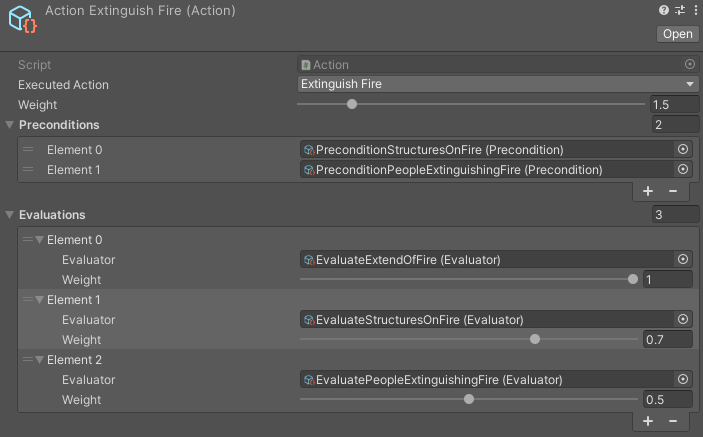
\includegraphics[scale=0.5]{images/utility_ai_scriptableobject_action.png}
	\caption{ScriptableObject for the extinguish fire action}
	\label{fig:utility_ai_scriptableobject_action}
\end{figure}

This is a ScriptableObject of the Action class, representing the extinguish fire action. At the top, the action to be performed and its weigh can be selected. Directly below this are the preconditions, in this example, the action to extinguish fire will only be considered if at least one structure is on fire and no one else is already doing this action. Finally, all the evaluations are listed, with each element consisting of an evaluator and its corresponding weight.

Using ScriptableObjects for actions has the advantage of allowing new preconditions and evaluators to be easily added within the Unity editor without the need for any additional coding. It's also clear which action has which components. The ScriptableObjects for the other utility AI elements look similar, but with different fields.

\newpage

\section{Examples}
\label{sec:utilityai_examples}
\subsection{Daily Routine}
\label{subsec:utilityai_realization_dailyroutine}

The first and simpler example shows an agent trying to live a normal daily routine. This routine consists of only three activities: working, eating and sleeping.

\begin{figure}[H]
	\centering
		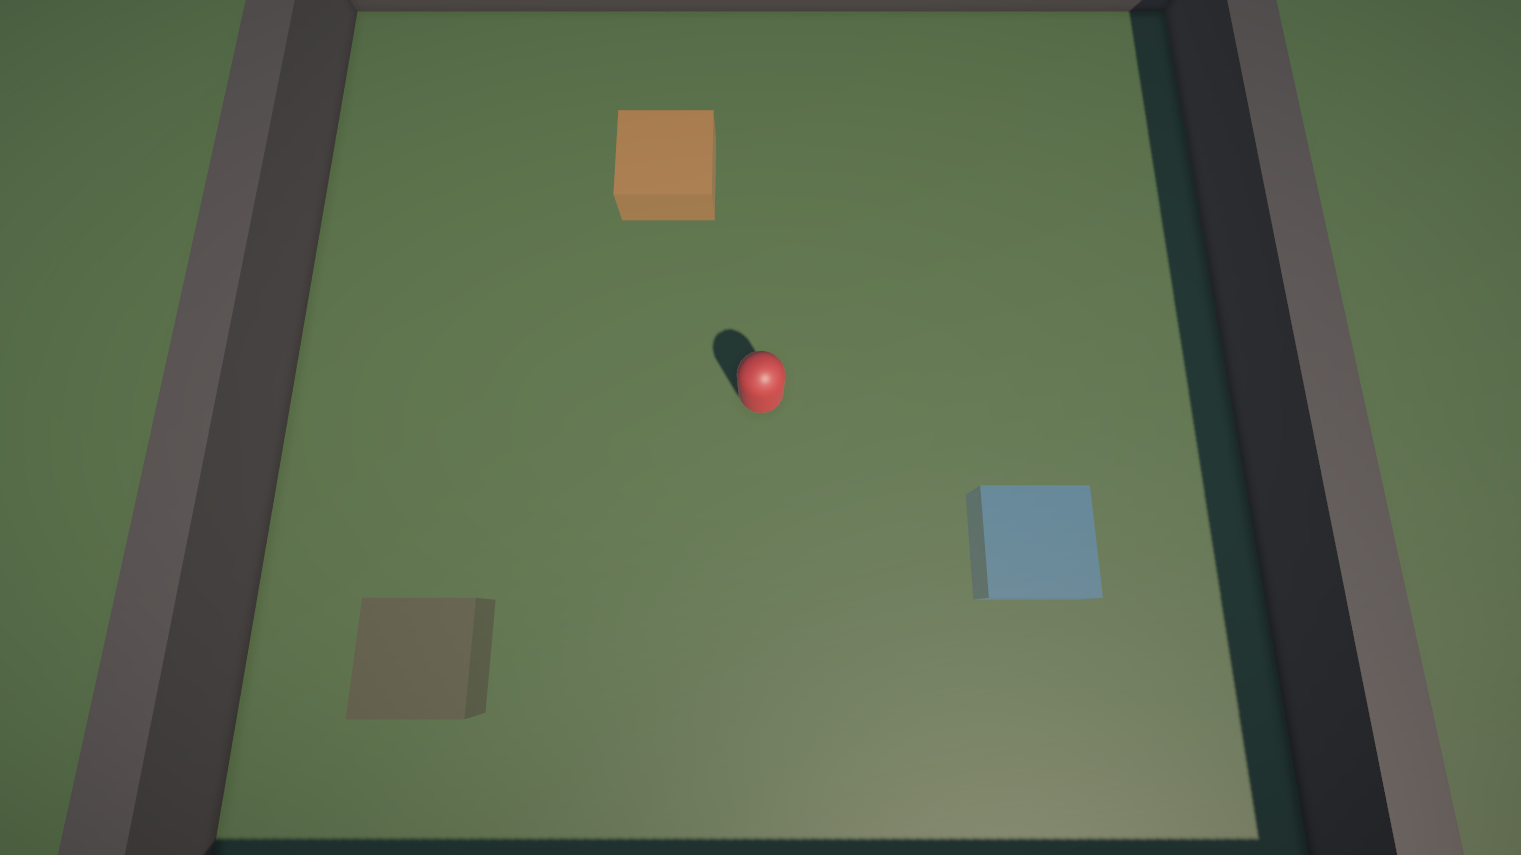
\includegraphics[scale=0.3]{images/utility_ai_scene_daily_routine.png}
	\caption{Scene in Unity for the agent's daily routine}
	\label{fig:utility_ai_scene_daily_routine}
\end{figure}

Each of these cubes represents a building in which the agent can perform a specific action: brown for working, orange for eating and blue for sleeping. Obviously, it can only do one action at a time, and it has to decide which one it wants to do by using the utility AI. The agent gradually loses saturation and energy over time, which can be regained by eating or sleeping. To eat, the agent must spend money on food, which it can earn by working. Sleeping and working both take time, while eating is instantaneous.

\begin{figure}[H]
	\centering
		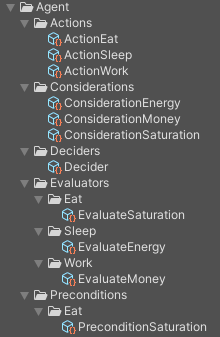
\includegraphics[scale=0.6]{images/utility_ai_daily_routine.png}
	\caption{Structure of the utility AI for the agent}
	\label{fig:utility_ai_daily_routine}
\end{figure}

The agent has three actions, each of which depends on only one evaluator. The action eat also has a precondition, which forbids the agent to eat if its saturation is above 90. With this structure, the agent is always able to choose the best action in this very simple world.

\newpage

\subsection{Spaceship}
\label{subsec:utilityai_realization_spaceship}

In this example, two spaceships with different elements on them are trying to attack each other. The following elements on the spaceships can be controlled by the two agents operating them:

\begin{tabular}{lp{12cm}}
Quarters: & The place where the agents sleep. \cr
Factories: & The place to produce materials that can be used as ammunition or to repair the ship. \cr
Storage: & The place where materials can be stored in larger quantities. \cr
Cannon: & The location from which the enemy spaceship can be fired at, using ammunition \cr
Fire Extinguisher: & The place where the fire extinguisher can be picked up to put out fires caused by enemy attacks.
\end{tabular}

There are also two other structures that are not intended to be operated by an agent:

\begin{tabular}{lp{12cm}}
Shields: & These elements are more resistant to enemy attack than any other structure. \cr
Paths: & The way for agents to walk from point A to point B.
\end{tabular}

\begin{figure}[H]
	\centering
		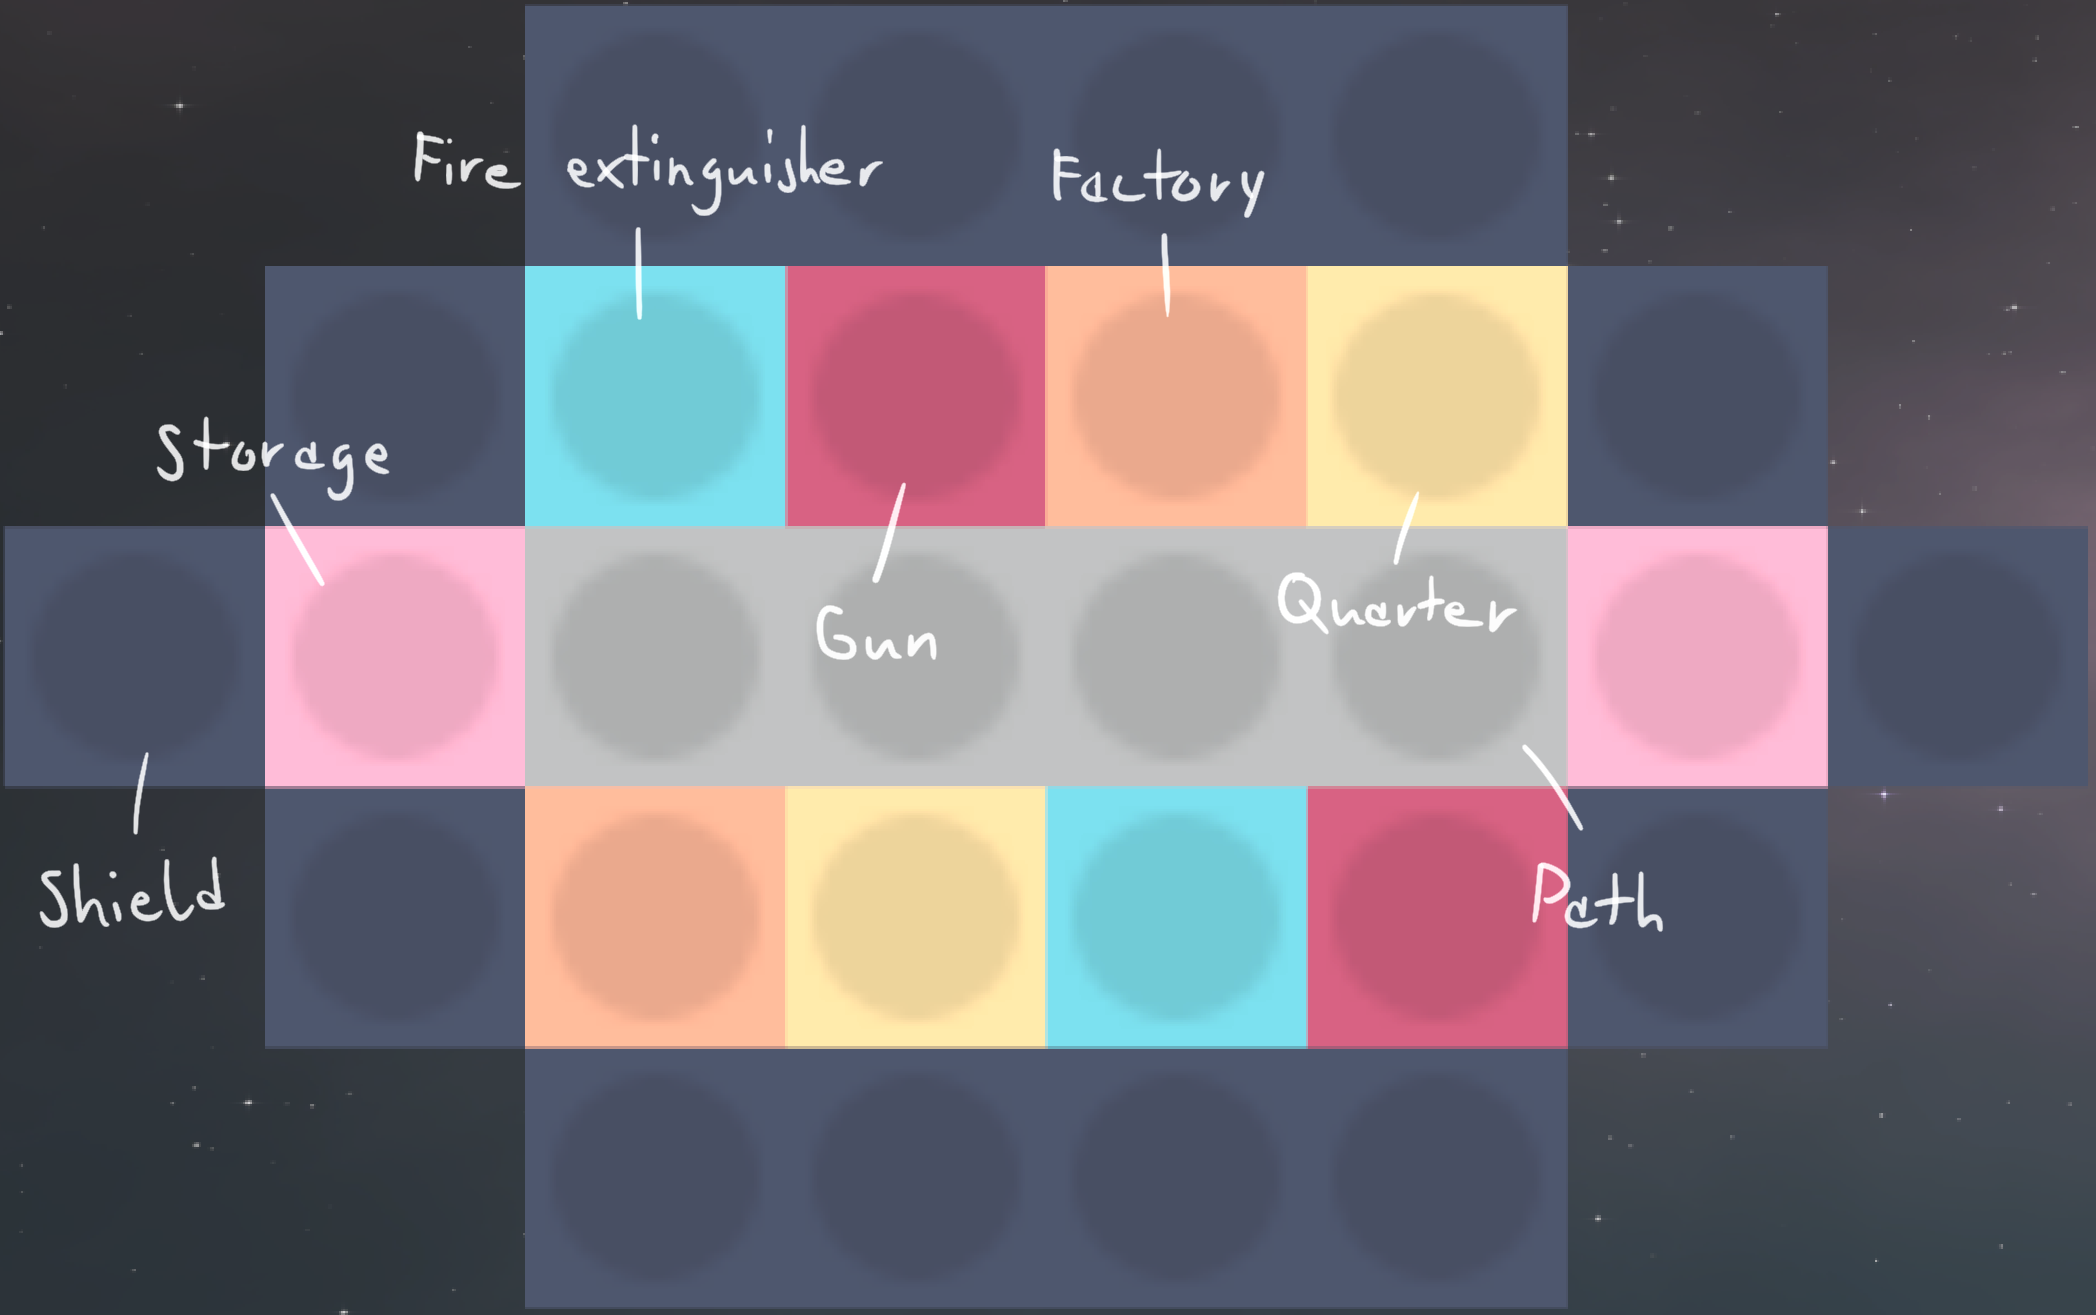
\includegraphics[scale=0.21]{images/utility_ai_scene_single_spaceship.png}
	\caption{Close up view of a single spaceship in Unity}
	\label{fig:utility_ai_scene_single_spaceship}
\end{figure}

In order for an agent to perform a certain action, it must first go to the specific structure. Once there, it can start performing the desired action. The agent can only use path elements to reach a new location, and navigation is done using Unity's NavMesh. Performing an action takes a fixed amount of time, which differs for each action.

A structure loses health points (HP) over time, depending on the extent of fire on that structure. Attacking the enemy spaceship means increasing the extent of fire on an enemy structure. Each shot increases the intensity by a certain amount. When a structure reaches 0 HP, it is marked as destroyed. Destroyed structures cannot be used to perform actions, but they can be repaired by taking some materials from the storage and using them to repair the structure.

\newpage

The actions available to the agent are shown in the following figure:

\begin{figure}[H]
	\centering
		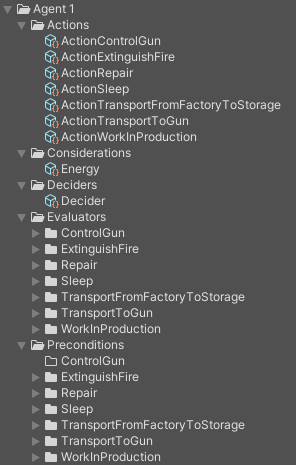
\includegraphics[scale=0.6]{images/utility_ai_spaceship.png}
	\caption{Structure of the utility AI for one agent}
	\label{fig:utility_ai_spaceship}
\end{figure}

To make it easier to understand, here is an example scenario: the agent starts by going to the factory to produce some materials. Once it's got some materials, it will choose to move those items to the warehouse, so that there's enough space in the factory to produce new items. After it has some items, it will move some of them to the cannon and start shooting at the enemy ship with the ammunition. At this point, it is likely that the enemy ship will start firing back as well, which will put the attacked structures on fire. The agent will then grab the fire extinguisher to defend his ship. If there are already destroyed structures, the agent might consider repairing them instead of doing other actions. It is also important to remember to sleep from time to time, otherwise its movement speed will be significantly reduced when it s too tired.

The spaceship will always have two copies of the same structure on board, as it is forbidden for more than one agent to perform the same action in the same place.

\begin{figure}[H]
	\centering
		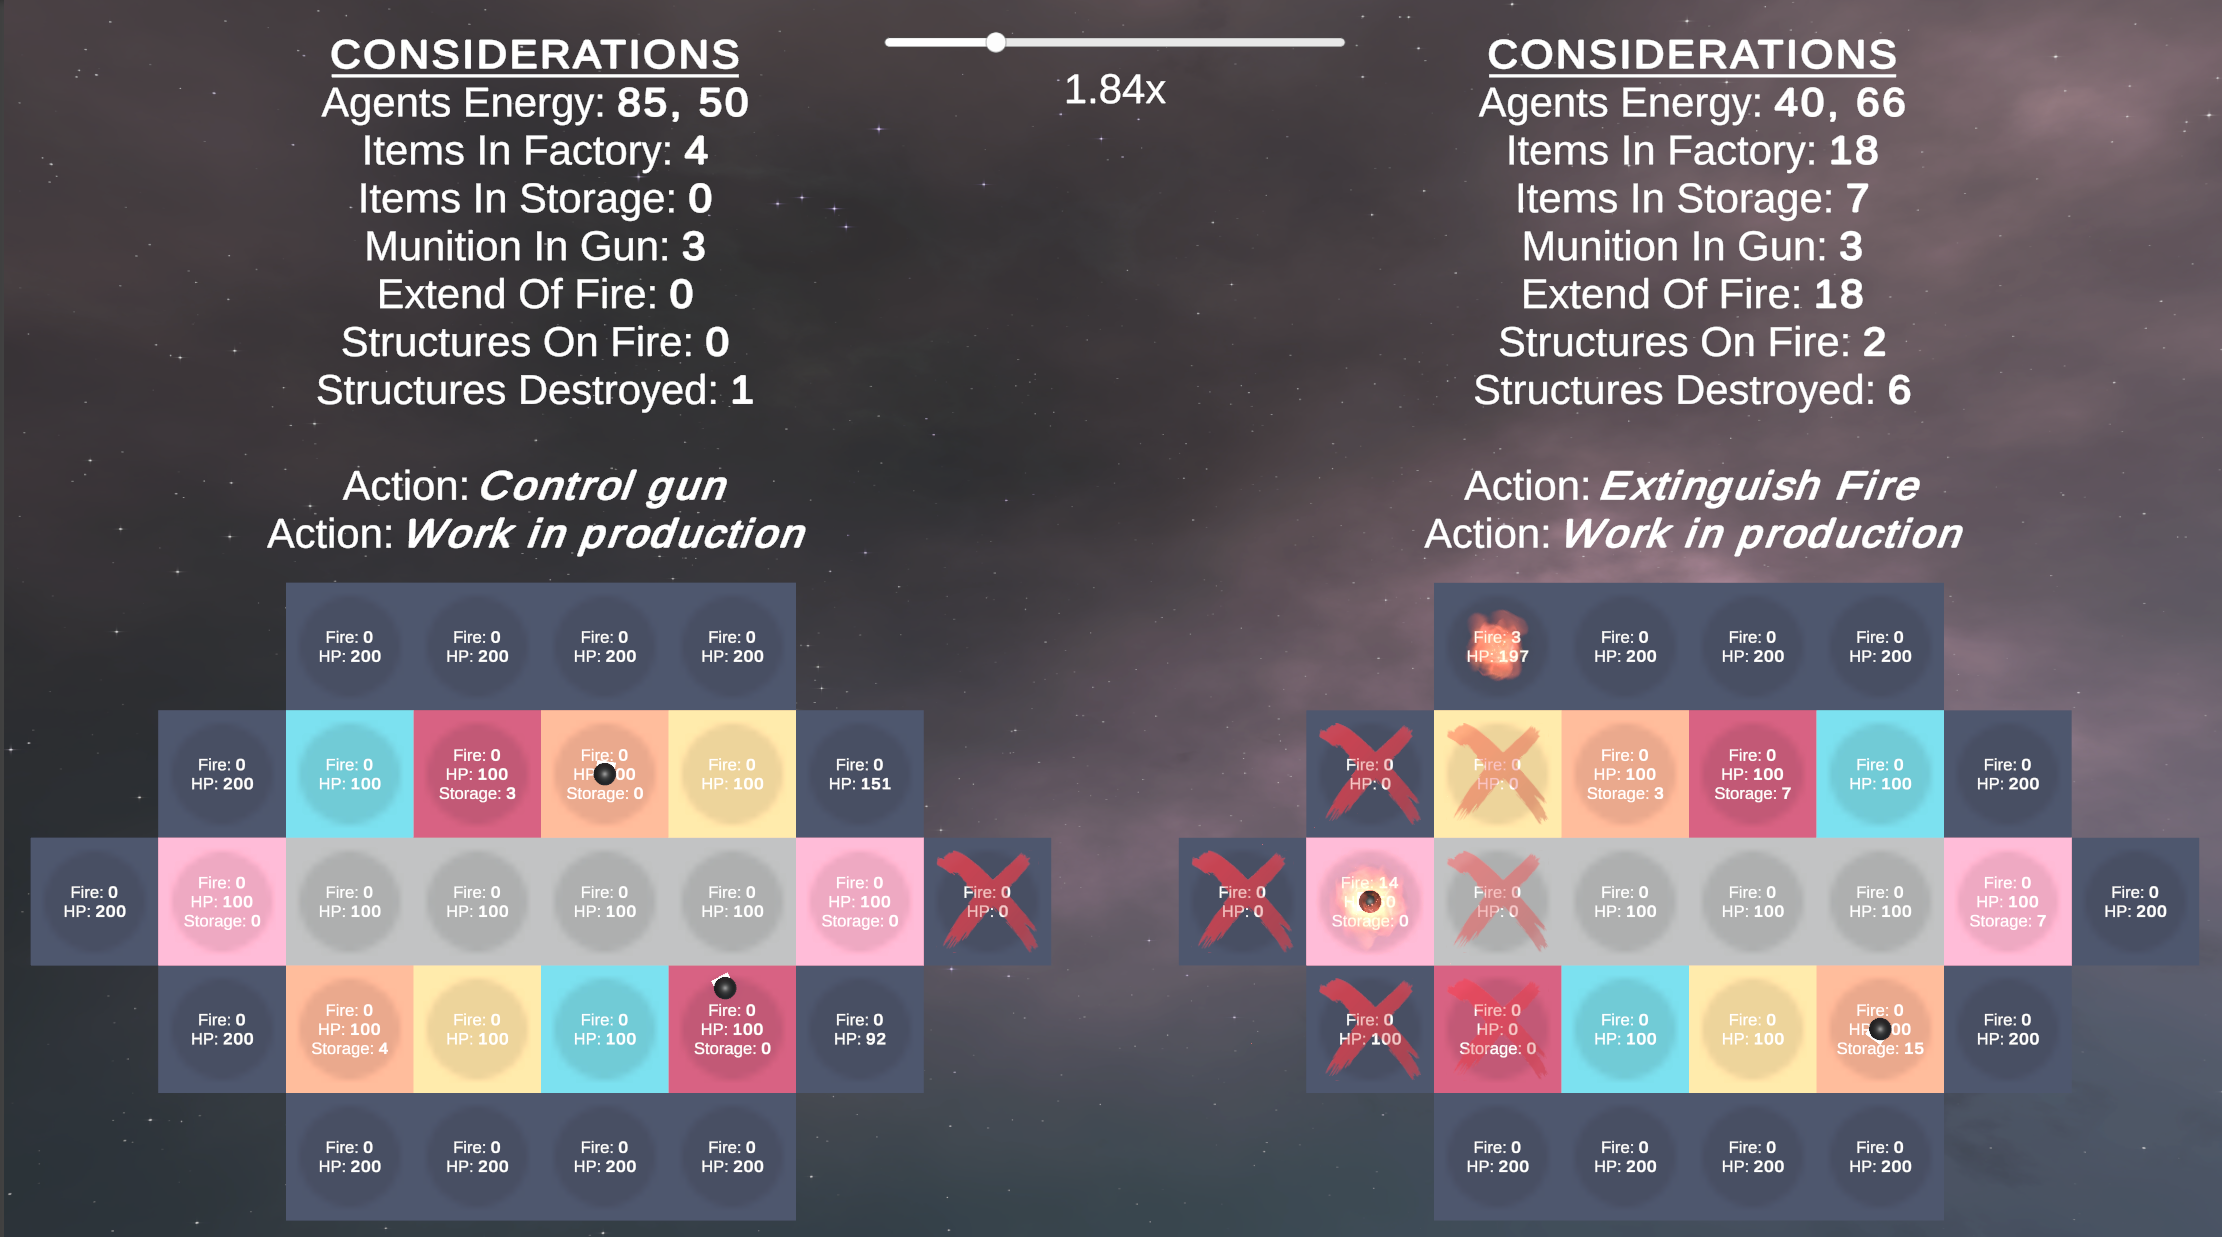
\includegraphics[scale=0.265]{images/utility_ai_scene_both_spaceship.png}
	\caption{Scene in Unity showing an ongoing battle}
	\label{fig:utility_ai_scene_both_spaceship}
\end{figure}

Figure \ref{fig:utility_ai_scene_both_spaceship} shows a screenshot of an ongoing battle between the two ships. At the top you can see the considerations of each spaceship, and just below them the current actions of the two agents. The crossed objects symbolise that they have been destroyed, and the burning ones are on fire. The extent of fire and its HP can be read in the overlay. It looks like the left spaceship is attacking, while the other is trying to defend itself by extinguishing fires and preparing materials for repair or counter-attack.

\newpage

\section{Strengths}
\label{sec:utilityai_strengths}

Utility AI is very good at making intelligent and realistic decisions based on the current state of the environment. It only lives in the present and doesn't care about what might happen afterwards. So utility AI becomes a very powerful tool when the agent has a lot of decisions to make and considerations to take into account, but doesn't have to worry about later decisions.

This tool also excels in its modularity. New actions can be added at any time during development without disturbing the others, and without having to change any of them to make them fit. The same goes for the evaluators. Because of the way the scores of the evaluators are calculated, new evaluators can be freely added to make the agent consider a new aspect of the game. This can be useful if, for example, a new feature has been added to the game during development, and the agent needs to take this into account when making a decision. It can also be very helpful when trying to find the most appropriate behaviour for an agent to be able to freely remove or add existing evaluators.

Thirdly, the weights of the actions combined with the weights of the evaluators can lead to very simple and fast changes in the behaviour of each agent. In the example of the defending agent from figure \ref{fig:utility_ai_sketch_defending_ai_with_values}, if the weights for the actions "heal" and "reload" are changed to 2 and "attack" to 3, the agent will play much more aggressively and will most likely change the order of the actions to "cover", "reload" and finally "attack". On the other hand, if the weight for the "attack" action is changed to 3 and its EH (enemy health) evaluator to 50\% weight, the AI will prioritise attacking enemy units with low health. Because it's so easy to change weights or even curves with just a few clicks, many different characters can be created from the same basic structure in no time, resulting in much more realistic and interesting NPCs.

\section{Weaknesses}
\label{sec:utilityai_weaknesses}

As mentioned previously, utility AI only considers its current environment and doesn't know what future actions might be. This makes it poor at planning ahead. This could be compensated by giving the NPC considerations that try to represent the future. However, since this consideration also depends on the action the NPC will choose, it will be very difficult to implement, and therefore isn't well supported by the framework.

It also struggles with sequential behaviour, like that of a tour guide. Since there are no states to switch to, all states would have to be represented by actions and considerations that change their value based on the current state. This would make the whole architecture more complex than it needs to be, whereas a simple FSM or behaviour tree would probably do the job.

\chapter{Goals for bachelor thesis}
\label{chap:goalsforbachelorthesis}

\section{Graphical implementation}
\label{sec:goalsforbachelorthesis_graphicalimplementation}

The main goal of the thesis is to make utility AI as intuitive and easy to use as possible. To achieve this, a graphical implementation of this framework might be the right choice. Each element would be represented by a node, similar to the behaviour tree in figure \ref{fig:behaviour_tree_tour_guide}. A final example of a graphical representation might look like the sketch in figure \ref{fig:utility_ai_sketch_defending_ai}. Making the whole structure node-based would give the user a much better overview because everything would be visible at once, which is currently not the case with the ScriptableObjects.

\section{Publish as an asset}
\label{sec:goalsforbachelorthesis_publishasanasset}

To make this tool accessible to everyone, not only does it need to be intuitive and easy to understand, but it also needs to be easy to find and incorporate into their current project. The Unity Asset Store seems like the perfect place to do this. Once uploaded, any Unity developer will be able to find and use it.

Of course, making this tool an asset takes time, as it cannot have bugs or other problems when it is published. A manual and some sample scenes to show the user how to use the utility AI would also be necessary. This will add an extra challenge to the thesis, but will also provide motivation to make it work flawlessly, which is always a good thing when developing a new tool.

\section{Improvements}
\label{sec:goalsforbachelorthesis_improvements}

The more utility AI was tested and played with, the more it became clear that this framework alone is not enough to make an AI work properly. The two example scenes in the section 4.6 both contain a state machine. That's because utility AI is able to decide the next best action, but it's not able to define the exact steps of how to execute that action.

Imagine an agent on a spaceship from section 4.6.2 needs to extinguish a fire. Utility AI would tell the agent to do this action, but this action is actually made up of four different actions:

\begin{tabular}{lp{12cm}}
1: & "walk to fire extinguisher" \cr
2: & "pick up fire extinguisher" \cr
3: & "walk to structure on fire" \cr
4: & "extinguish fire"
\end{tabular}

All of these actions must be performed in a specific order, and most of them must wait for a condition to occur before the next action can be executed. For example, the second action needs to wait for the agent to arrive before it can pick up the fire extinguisher. Simply calling an action script, which is what the utility AI does, is not enough.

The resulting idea is to use utility AI for the high-level decision making, while combining it with another tool that helps to execute the actions one at a time. These actions may not always be in a sequence, as in the example of extinguishing a fire. A decision might also be something like entering a house, where the agent might need a behaviour like the one in figure 3.1 to walk through a door.

\newpage

There are different ways of defining the exact execution of actions: state machines work very well, as the complexity of declaring the behaviour of a single action is usually not very complex. Another way is to use a behaviour tree to allow more complex behaviour, such as walking through a door. And interestingly, GOAP could also work because it's input is a goal and it generates a sequence of actions. So utility AI could decide the next goal for the agent, while GOAP plans how to execute it.

Because there are so many possibilities, more research and testing will presumably be needed in the thesis. Nevertheless, in order to keep it generic, it might be a good idea to give the user the option to use a tool of their choice for this purpose. An implementation of a behaviour tree, for example, could also be packaged in this tool, so that the user could get started immediately after obtaining this asset.